\begin{center}
\begin{tikzpicture}
    \node[anchor=south west,inner sep=0] (image)  at (0,0) {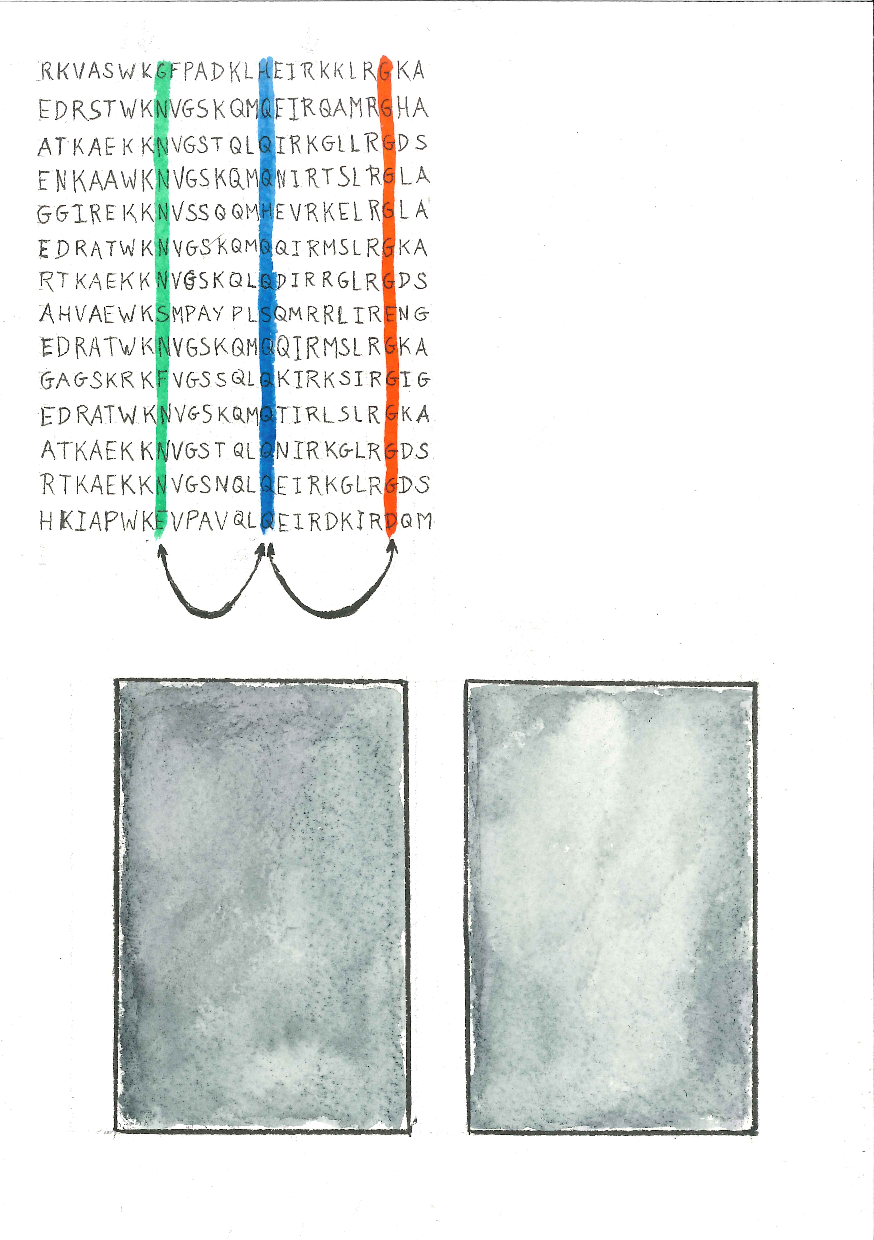
\includegraphics[trim={2mm, 2mm, 2mm, 2mm}, width=0.995\pagewidth]{scans/pg_0003.pdf}};

    \begin{scope}[x={(image.south east)},y={(image.north west)}]
        \if\helplines1
        	\draw[help lines,xstep=.1,ystep=.1] (0,0) grid (1,1);
        \fi
        \node[align=justify, anchor=north west, text width = 0.36\pagewidth](0) at (0.57, 0.95) {\english{If we search for similar proteins in our databases of sequences and align them by similarity, we find that when a column - that is, a position - changes, usually other columns change as well.
        This is how we can predict contacts.}};
        
        \node[align=justify, anchor=north west, text width = 0.36\pagewidth](0) at (0.57, 0.73) {\spanish{Si buscamos proteínas similares en nuestras bases de datos de secuencias y las alineamos por similitud, encontraremos que cuando una columna - es decir, una posición - cambia, normalmente otras cambian también.
        Así es como podemos predecir contactos.}};
        
        \draw[fill=white, opacity=0.4] (0.125,0.08) -- (0.465,0.08) -- (0.46,0.448) -- (0.125, 0.45) -- cycle;
        \draw[fill=white, opacity=0.4] (0.538,0.08) -- (0.87,0.08) -- (0.87,0.448) -- (0.538, 0.45) -- cycle;
        \node[align=justify, anchor=north west, text width=0.28\pagewidth] at (0.15, 0.40)
        {\english{Technical note: if green is in contact with blue, and blue is in contact with orange, we will see a correlation between blue and orange. Distinguishing the true correlations from the spurious ones is the core of my research.}};
        
        \node[align=justify, anchor=north west, text width=0.28\pagewidth] at (0.55, 0.40)
        {\spanish{Nota técnica: si verde está en contacto con azul, y azul está en contacto con naranja, veremos una correlación entre azul y naranja. Distinguir entre las correlaciones verdaderas y espúrias es el eje de mi investigación.}};
    \end{scope}

\end{tikzpicture}
\end{center}